%%%%%%%%%%%%%%%%%%%%%%%%%%%%%%%%%%%%%%%%%%%%%%%%%%%%%%%%%%
\section{Generalizing the Technique}
\label{sec:generalizing}
%%%%%%%%%%%%%%%%%%%%%%%%%%%%%%%%%%%%%%%%%%%%%%%%%%%%%%%%%%
Synoptic is only one of the many algorithms used to infer models from
executions.  These techniques are difficult to compare and nearly impossible
to combine.  Some are slow, and some produce models that may not
be minimal. 

One of the advantages of the InvariMint approach is that it
provides a way to compare and combine different model inference approaches on the
same terms, and does so in an efficient, deterministic way.
In this section, we will first describe kTails ~\cite{kTailsOrigin}, a widely
used algorithm for FSM inference. We will then illustrate how kTails can
be expressed by composing invariant DFAs. We argue that InvariMint offers a
unifying framework for model inference methods by characterizing the existing
techniques in terms of invariant DFAs.


%%%%%%%%%%%%%%%%%%%%%%%%%%%%%%%%%%%%%%%%%%%%%%%
\subsection{kTails}
%%%%%%%%%%%%%%%%%%%%%%%%%%%%%%%%%%%%%%%%%%%%%%%

kTails is a coarsening algorithm for inferring concise models.
The algorithm begins with a fine-grained representation of a model in
which each event instance (not event type) is mapped to its own partition as in
Figure~\ref{fig:ktails}a.

kTails then iteratively merges pairs of
k-equivalent partitions. These are partitions in the model that are roots of
identical sub-graphs 
up to depth k. The resulting graphs after applying $k = 0$ and $k = 1$ to the
model in Figure~\ref{fig:ktails}a are shown in ~\ref{fig:ktails}b and
~\ref{fig:ktails}c respectively. 

The initial kTails graph is analogous to a trace graph for Synoptic in which
each execution trace from the input logs is a single path from the INITIAL to
TERMINAL nodes. It is possible to infer Synoptic-style models by simply applying
kTails to a trace graph for arbitrary values of k. Synoptic's initial model, in
which all events of the same type are merged, is
equivalent to running kTails on the trace graph with $k = 0$.

%%%%%%%%%%%%%%%%%%%%%%%%%%%%%%%%%%%%%%%%%%%%%%%
\subsection{Representing kTails using InvariMint}
%%%%%%%%%%%%%%%%%%%%%%%%%%%%%%%%%%%%%%%%%%%%%%%


\begin{figure}
   \center
   {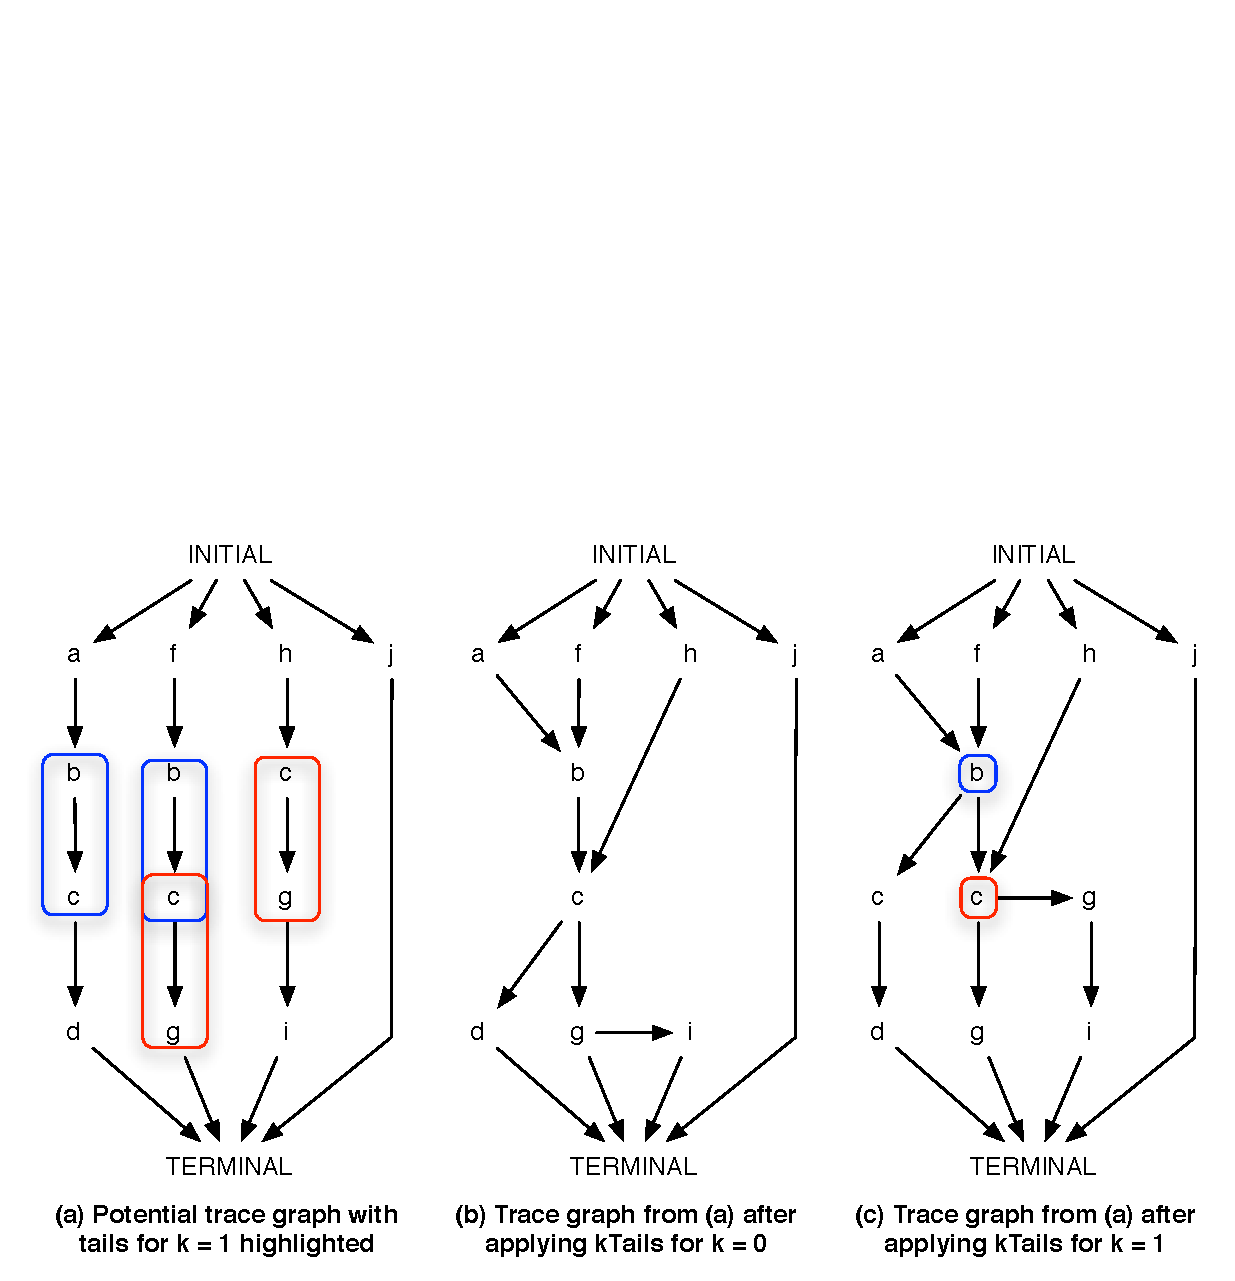
\includegraphics[width=0.95\columnwidth]{fig/ktails.pdf}}
   \caption{A sample trace graph and its corresponding models using
   InvariMint for kTails for k = 0 and k = 1.}
   \label{fig:ktails}
\end{figure}


\begin{figure}
   \center
   {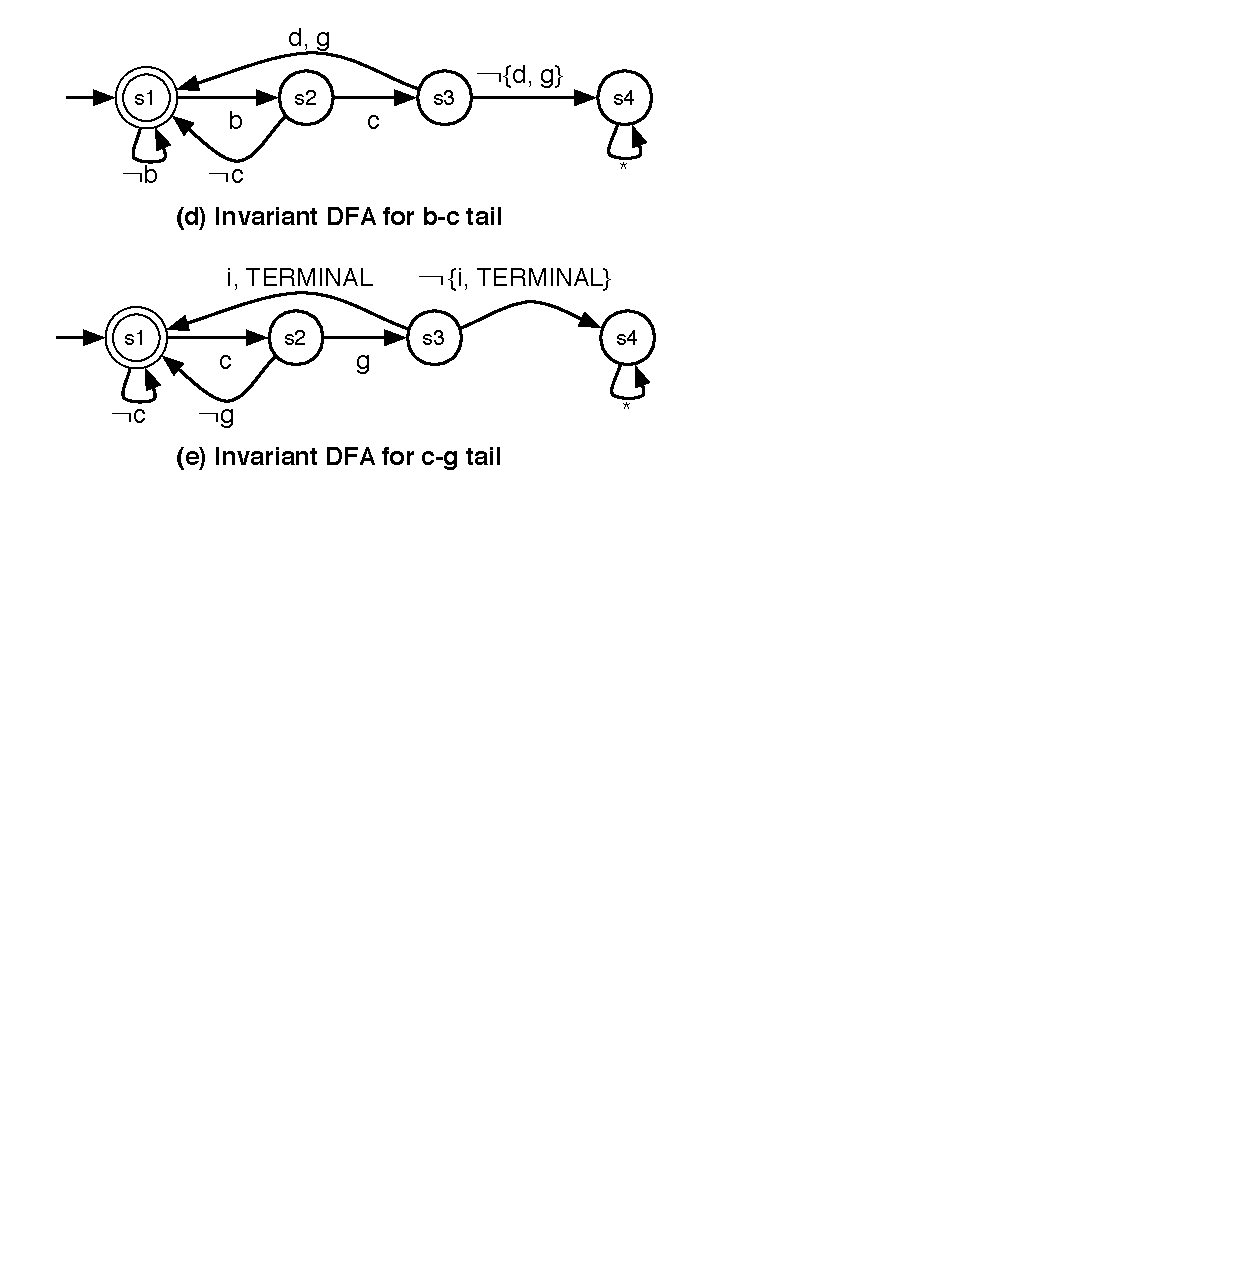
\includegraphics[width=0.95\columnwidth]{fig/tails.pdf}}
   \caption{Invariant DFAs for the tails in Figure~\ref{fig:ktails}a for
   $k = 1$.}
   \label{fig:tails}
\end{figure}


When k = 0, kTails merges all event instances of the same type which is
precisely equivalent to Synoptic's initial model and can be constructed with
InvariMint using the \emph{Never Immediately followed by} invariants. An example
of this is shown in Figure~\ref{fig:ktails}b.

For $k > 0$, invariants can describe tails of length k in
the model. To construct these, we mine all sub-graphs of depth $k + 1$ in the initial graph
that are shared by \textbf{at least two traces}. For all such tails, the set of
events that can immediately follow the tail are also recorded.
Each sub-graph is then translated into
an invariant DFA which stipulates that if a tail is seen, it must be immediately followed by
one of the next possible follow events. Figure~\ref{fig:tails} illustrates
these DFAs for $k = 1$.

Using these translation mechanisms, InvariMint is able to express the key properties
of kTails simply by taking the
intersection of all immediate invariants and each of the tail
invariants.

InvariMint offers a unifying framework for inferring models from executions by 
reducing other inference techniques to the set of invariants
that describe the essential properties of their models. Because these invariants
are all describable with formal languages,
it is possible to generalize, combine, and compare existing
techniques simply by adjusting the set of invariants used to construct the final
model.

For example, using InvariMint a developer would be able to merge k-tails of
varying length depending on the event type, and could intersect that model with
whichever temporal Synoptic invariants deemed most appropriate. This flexibility
provides a way for developers to better explore the space of formal
specification and to quickly create customized hybrid inference algorithms.
